\documentclass[11pt,a4paper]{article}
\usepackage{paquete}


\begin{document}


\pagestyle{fancy}
%\renewcommand{\sectionmark}[1]{\markboth{}{\thesection\ \ #1}}
\lhead{\sc }
\chead{}
\rhead{\rightmark}
\lfoot{}
\cfoot{}
\rfoot{\thepage}

%\begin{comment}
%
% Carátula:

\begin{titlepage}

\thispagestyle{empty}

\begin{center}

\includegraphics[scale=0.5]{./figuras/logo_utn}\\
\hfill \newline
\large{\textsc{Resumen Paradigma Funcional}}\\
\large{\textsc{Facultad Regional Buenos Aires}}\\
\large{\textsc{Universidad Tecnologica Nacional}}\\
\end{center}

% \newline
\begin{center}
\LARGE{\textsc{Paradigmas de Programación -- $K2032$}}\\
\hfill \newline
\huge{Trabajos Prácticos}
\end{center}

\vspace{2cm}



\begin{center}
	\begin{tabular}{lc}
		PAZ PORTILLA, José Miguel & \ \ \ 2028244 \\
		\texttt{\href{mailto:jpazportilla@frba.utn.edu.ar}{jpazportilla@frba.utn.edu.ar}}\\
	\end{tabular}
\end{center}

\vspace{1cm}
\begin{center}
\large{\today}
\end{center}

\end{titlepage}

%
% Pongo el índice en una página aparte:
%
{
  \hypersetup{linkcolor=black}
  \tableofcontents
}
% \tableofcontents
\thispagestyle{empty}
\newpage
%
% Hago que las páginas se comiencen a contar a partir de aquí:
%
\setcounter{page}{1}



\newpage
%%%%%%%%%%%%%%%%%%%%%%%%%%%%%%%%%%%%%%%%%%%%%%%%%%%%%%%%%%%%%%%%%%%%%%%

\section{Introducción a Objetos -> Video 17 Youtube}
En este paradigma de objetos se vuelve a tener efecto, pero es menos declarativo que funcional y lógico. Se utiliza el lenguaje de programación Wollok. La idea es combinar estructuras de datos y operaciones.

Las caracteristicas de un objeto son:

\begin{enumerate}
	\item Exponen una interfaz, es un conjunto de operaciones con las que se pueden interactuar con el objetos. Solo se puede interactuar con objetos mediantes mensajes. Los mensajes que un objeto entiende va a ser el resultado de poseer metodos.
	\item Pueden llegar a tener estado interno, que son atributos, es decir referencias a otros objetos. Estos atributos pueden cambiar de referencia y apuntar a otros objetos.
	\item Tienen una identidad, cada objeto es diferente a cualquier otro, aunque hayan otros que respondan a los mismos mensajes y estado interno.
\end{enumerate}

\subsection{Problema: La Golondrina Pepita}

\begin{itemize}
	\item Un ornitólogo nos pide ayuda para estudiar el Consumo de Energía de la golondrina Pepita
	\item El Volar consume energia de Pepita.
	\item El Comer recupera la energía de Pepita.
\end{itemize}

\subsubsection{Resolución: La Golondrina Pepita}
\begin{itemize}
	\item La palabra object define un objeto nuevo.
	\item La palabra var define un atributo que podrá ser cambiado
	\item La palabra method permite crear métodos.
	\item El metodo volar() y comer() causan efecto.
	\item El metodo energia() son solo de consulta.
\end{itemize}

\subsubsection{Wollok: La Golondrina Pepita}
\lstinputlisting[language=java]{codigos/video17_e1_pepita/src/pepita.wlk}

\subsection{Problema: La entrenadora de aves Emilia}
\begin{itemize}
	\item Emilia solo sabe entrenar aves
	\item La aves deben comer 5g, volar 10km y volver a comer 5g.
\end{itemize}

\subsubsection{Resolución: La entrenadora de aves Emilia}
\begin{itemize}
	\item Emilia no conoce a Pepita, pero como Pepita entiende los mensajes come y vola, entonces podra entrenarla.
\end{itemize}

\subsubsection{Wollok: La entrenadora de aves Emilia}
\lstinputlisting[language=java]{codigos/video17_e1_pepita/src/emilia.wlk}

\subsection{Emilia entrena a Pepita}
Emilia puede entrenar a cualquier objeto que entienda los mensajes come y vola. En la \autoref{fig:test emilia entrena a pepita} se observa que pepita sufre el efecto luego que emilia la entrena, aumentando su energia de $100J$ a $180J$.


\subsubsection{Wollok: Emilia entrena a Pepita}
\lstinputlisting[language=java]{codigos/video17_e1_pepita/src/test_emilia_pepita.wtest}

\begin{figure}[H]
	\centering
	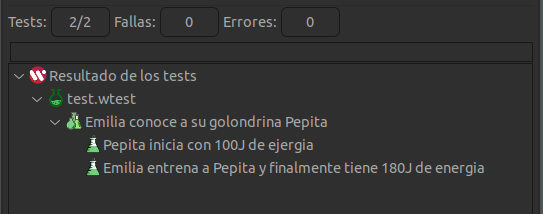
\includegraphics[scale=0.7]{figuras/test_pepita_emilia.png}
    \caption{Test unitario de pepita siendo entrenada por emilia.}
    \label{fig:test emilia entrena a pepita}
\end{figure}  

\subsection{Conceptos clave de la programación orientada a objetos}
\begin{enumerate}
	\item Los objetos están encapsulados ya que oculta y protege de los detalles de su implementación. Solo veo la interfaz de un objeto, o sea que mensajes entiende. Solo nos intereza saber que puede hacer. No puedo ver, ni usar los atributos de un objeto, sólo un objeto puede manipular sus atributos.
	\item Cuando se delega en un objeto alguna actividad, se le da la responsabilidad al objeto de saber como hacerlo mientras que lo termine haciendo.
	\item El polimorfismo implica que un objeto que envia mensajes pueda manipular al menos a dos objetos, siempre y cuando ellos entiendan los mensajes que envia el objeto.
\end{enumerate}
\subsection{Otra ave: El hancón pepote}
Pepote es otra ave ya que entiende los mismos mensajes que Pepita, es decir come y vola. Para emilia que sabe entrenar aves le es indiferente cual de ellos debe entrenar. Pepote causa efecto sobre su energia al volar y comer, pero lo hace de forma distinta a Pepita.
Se observa que su tiene como atributos a comido y volado, ademas su metodo energia no es un getter, sino que devuelve el resultado una operación.
\subsection{Wollok: El hancón pepote}
\lstinputlisting[language=java]{codigos/video17_e1_pepita/src/pepote.wlk}

\subsection{Wollok-Test: Emilia entrena a Pepote}
\lstinputlisting[language=java]{codigos/video17_e1_pepita/src/test_emilia_pepote.wtest}

\begin{figure}[H]
	\centering
	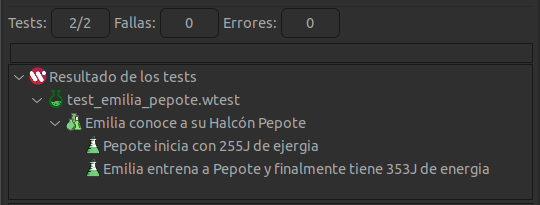
\includegraphics[scale=0.7]{figuras/test_pepote_emilia.png}
    \caption{Test unitario de pepote siendo entrenado por emilia.}
    \label{fig:test emilia entrena a pepote}
\end{figure}  

\subsection{Diseño de métodos para favorecer el polimorfismo entre objetos}

Si se tiene un objeto Pepaza que entiende los mensajes:

\begin{itemize}
	\item come()
	\item volar(kilometros)
	\item nadar()
\end{itemize}

Emilia no la podrá entrenar ya que 	Pepaza no entiene el mensaje vola, sino volar. Además su metodo come no espera un parametro que indique la cantidad que debe comer.
Solución cambiar volar por vola y agregar parametro gramos en el metodo come aunque no se use.

Si se tiene otro objeto Pepudo que entiende los mensajes:

\begin{itemize}
	\item come()
	\item nada()
\end{itemize}

Emilia tampoco lo podrá entrenar a Pepudo, ya que no entiende el mensaje vola. 

\subsection{Otro entrenado Ramiro}
Ramiro en otro entrenado de aves. Si esta de buen humor hace volar a las aves 15km, sino 30km. Se sabe que si duerme por lo menos 8 horas entonces esta de buen humor, sino no.
\subsection{Resolución: Otro entrenado Ramiro}
Por ser entrenador, debe enterder el mensaje entrena que tiene un ave como parametro. Ademas tiene un atributo variable que indica las horas que durmio. Lo inicio en 0 horas dormida y entonces esta de mal humor. Si entreda a Pepita o Pepote los hara volar 30km, pero si en cambien durmio al menos 8 horas, entonces solo hará volar al ave que entrene 15km

\subsection{Wollok: Otro entrenador Ramiro}
\lstinputlisting[language=java]{codigos/video17_e1_pepita/src/ramiro.wlk}

\subsection{Wollok-Test: Ramiro entrena a Pepita y Pepote, con buen y mal humor}
\lstinputlisting[language=java]{codigos/video17_e1_pepita/src/test_ramiro_pepita_pepote.wtest}

\begin{figure}[H]
	\centering
	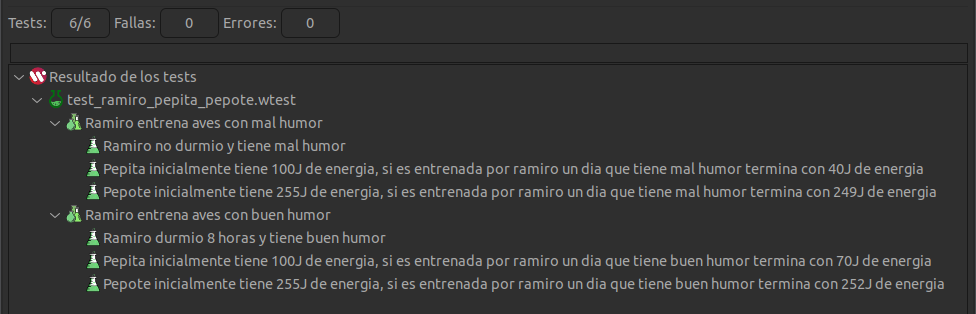
\includegraphics[scale=0.5]{figuras/test_ramiro_pepita_pepote.png}
    \caption{Test unitario de ramiro entrenado con buen y mal humor a pepita y pepote.}
    \label{fig:test ramiro entrena a pepita y pepote}
\end{figure}  

%%%%%%%%%%%%%%%%%%%%%%%%%%%%%%%%%%%%%%%%%%%%%%%%%%%%%%%%%%%%%%%%%%%% 
\newpage
\section{Práctica: La Feria -> Video 18 Youtube}

Julieta cuenta con tickets y ademas no está cansada. Va a jugar los distintos juegos de la feria y al finalizar termina con más tickets y cansada dependiendo de cada juego.

\subsection{Wollok: Jugadores de la feria}
\lstinputlisting[language=java]{codigos/Video18_e1_la_feria/src/jugadores.wlk}

\subsection{Wollok: Juegos de la feria}
\lstinputlisting[language=java]{codigos/Video18_e1_la_feria/src/juegos.wlk}

\subsection{Wollok: Premio de la feria}
\lstinputlisting[language=java]{codigos/Video18_e1_la_feria/src/premios.wlk}


\subsection{Wollok-Test: Julieta juega en la feria}
\lstinputlisting[language=java]{codigos/Video18_e1_la_feria/src/test_julieta_juega_en_la_feria.wtest}

\begin{figure}[H]
	\centering
	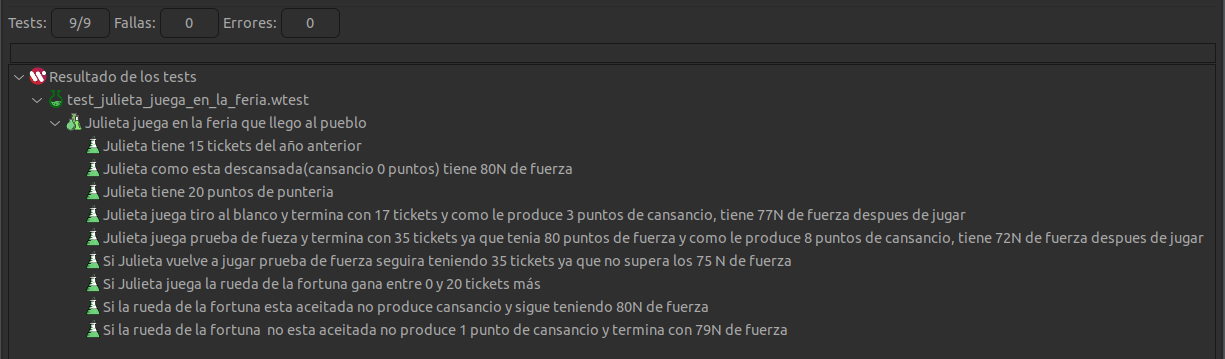
\includegraphics[scale=0.4]{figuras/test_julieta_juega_en_la_feria.png}
    \caption{Test unitario julieta juega en la feria.}
    \label{fig:test julieta juega en la feria}
\end{figure}  

%%%%%%%%%%%%%%%%%%%%%%%%%%%%%%%%%%%%%%%%%%%%%%%%%%%%%%%%%%%%%%%%%%%% 
\newpage
\section{Clases como plantillas para crear objetos -> Video 19 Youtube}

Las clases no son objetos, solo son sus moldes a partir de ellos se pueden crear objetos mediante una instanciación.
La clases definen atributos y prevee metodos. No se le pueden mandar mensajes a las clases ya que no son objetos.
Todos los objetos de una misma clase son polimorficos ya que entienden los mismos mensajes.

\subsection{Wollok: Clase Golondrina}
\lstinputlisting[language=java]{codigos/Video19_e1_ClaseGolondrina/src/golondrina.wlk}

\subsection{Wollok-Test: Clase Golondrina}
\lstinputlisting[language=java]{codigos/Video19_e1_ClaseGolondrina/src/test_golondrina.wtest}

\begin{figure}[H]
	\centering
	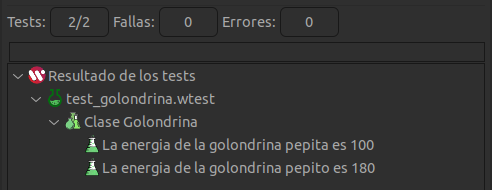
\includegraphics[scale=0.4]{figuras/test_clase_golondrina.png}
    \caption{Test unitario clases golondrina.}
    \label{fig:test clase golondrina}
\end{figure} 

%%%%%%%%%%%%%%%%%%%%%%%%%%%%%%%%%%%%%%%%%%%%%%%%%%%%%%%%%%%%%%%%%%%% 
\newpage
\section{Colecciones y Bloques -> Video 20 Youtube}

\subsection{Lista}
Las listas se representas como: \textit{const lista = new [1,2,3]}\\
 
Operaciones de Listas 

\begin{figure}[H]
	\centering
	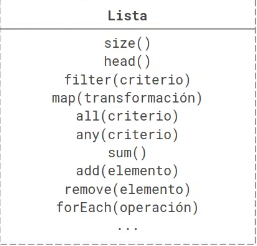
\includegraphics[scale=0.5]{figuras/operaciones_listas.png}
    \caption{Operaciones de las listas.}
    \label{fig:operaciones de listas}
\end{figure} 

De consulta son:

\begin{itemize}
	\item size()
	\item head()
	\item filter(criterio)
	\item map(criterio)
	\item all(criterio)
	\item any(criterio)
	\item sum()
\end{itemize}

y de efecto:

\begin{itemize}
	\item add(elemento)
	\item remove(elemento)
	\item forEach(operacion)
\end{itemize}

\subsection{Wollok: Clase Vaca}
\lstinputlisting[language=java]{codigos/Video20_e1_Animales/src/vaca.wlk}

\subsection{Wollok: Clase Cabra}
\lstinputlisting[language=java]{codigos/Video20_e1_Animales/src/cabra.wlk}

\subsection{Wollok: Clase Corral}
\lstinputlisting[language=java]{codigos/Video20_e1_Animales/src/corral.wlk}

\subsection{Wollok-Test: Prueba en lista de vacas}
\lstinputlisting[language=java]{codigos/Video20_e1_Animales/src/test_vacas.wtest}
%%%%%%%%%%%%%%%%%%%%%%%%%%%%%%%%%%%%%%%%%%%%%%%%%%%%%%%%%%%%%%%%%%%% 
\newpage
\section{Herencia -> Video 21 Youtube}
Las subclases heredan atributos y metodos de una superclase. Cada subclase tiene una sola superclase. No hace falta tener herencia para tener polimorfismo.

\subsection{Wollok: Clase Tanque}
\lstinputlisting[language=java]{codigos/Video21_e1_TanquesDeGuerra/src/tanque.wlk}

\subsection{Wollok: Clase Arma}
\lstinputlisting[language=java]{codigos/Video21_e1_TanquesDeGuerra/src/arma.wlk}

%%%%%%%%%%%%%%%%%%%%%%%%%%%%%%%%%%%%%%%%%%%%%%%%%%%%%%%%%%%%%%%%%%%% 
\newpage
\section{Herencia vs Composicion -> Video 22 Youtube}

\subsection{Wollok: Juego Por La Horda}
\lstinputlisting[language=java]{codigos/Video22_e1_PorLaHorda/src/juego.wlk}

%%%%%%%%%%%%%%%%%%%%%%%%%%%%%%%%%%%%%%%%%%%%%%%%%%%%%%%%%%%%%%%%%%%% 
\newpage
\section{Manejo de Errores -> Video 23 Youtube}

\subsection{Wollok: Clase Impresora}
\lstinputlisting[language=java]{codigos/Video23_e1_ErroresImpresiones/src/impresora.wlk}

\subsection{Wollok: Clase Cabezal}
\lstinputlisting[language=java]{codigos/Video23_e1_ErroresImpresiones/src/cabezal.wlk}

\subsection{Wollok: Clase Cartucho}
\lstinputlisting[language=java]{codigos/Video23_e1_ErroresImpresiones/src/cartucho.wlk}

%%%%%%%%%%%%%%%%%%%%%%%%%%%%%%%%%%%%%%%%%%%%%%%%%%%%%%%%%%%%%%%%%%%% 
\newpage
\section{Parcial Monetizaciones-> Video 24 Youtube}

\subsection{Wollok: Contenidos}
\lstinputlisting[language=java]{codigos/Video24_Parcial_Monetizacion/src/contenido.wlk}

\subsection{Wollok: Monetizaciones}
\lstinputlisting[language=java]{codigos/Video24_Parcial_Monetizacion/src/monetizaciones.wlk}

\subsection{Wollok: Usuarios}
\lstinputlisting[language=java]{codigos/Video24_Parcial_Monetizacion/src/usuarios.wlk}

%%%%%%%%%%%%%%%%%%%%%%%%%%%%%%%%%%%%%%%%%%%%%%%%%%%%%%%%%%%%%%%%%%%% 
\newpage
\section{Parcial Super Computadora-> Video 25 Youtube}

\subsection{Wollok: Computadoras}
\lstinputlisting[language=java]{codigos/Video25_Parcial_Computadoras/src/computadoras.wlk}

\subsection{Wollok: Modos de trabajo}
\lstinputlisting[language=java]{codigos/Video25_Parcial_Computadoras/src/modos.wlk}

%%%%%%%%%%%%%%%%%%%%%%%%%%%%%%%%%%%%%%%%%%%%%%%%%%%%%%%%%%%%%%%%%%%% 
\newpage
\appendix
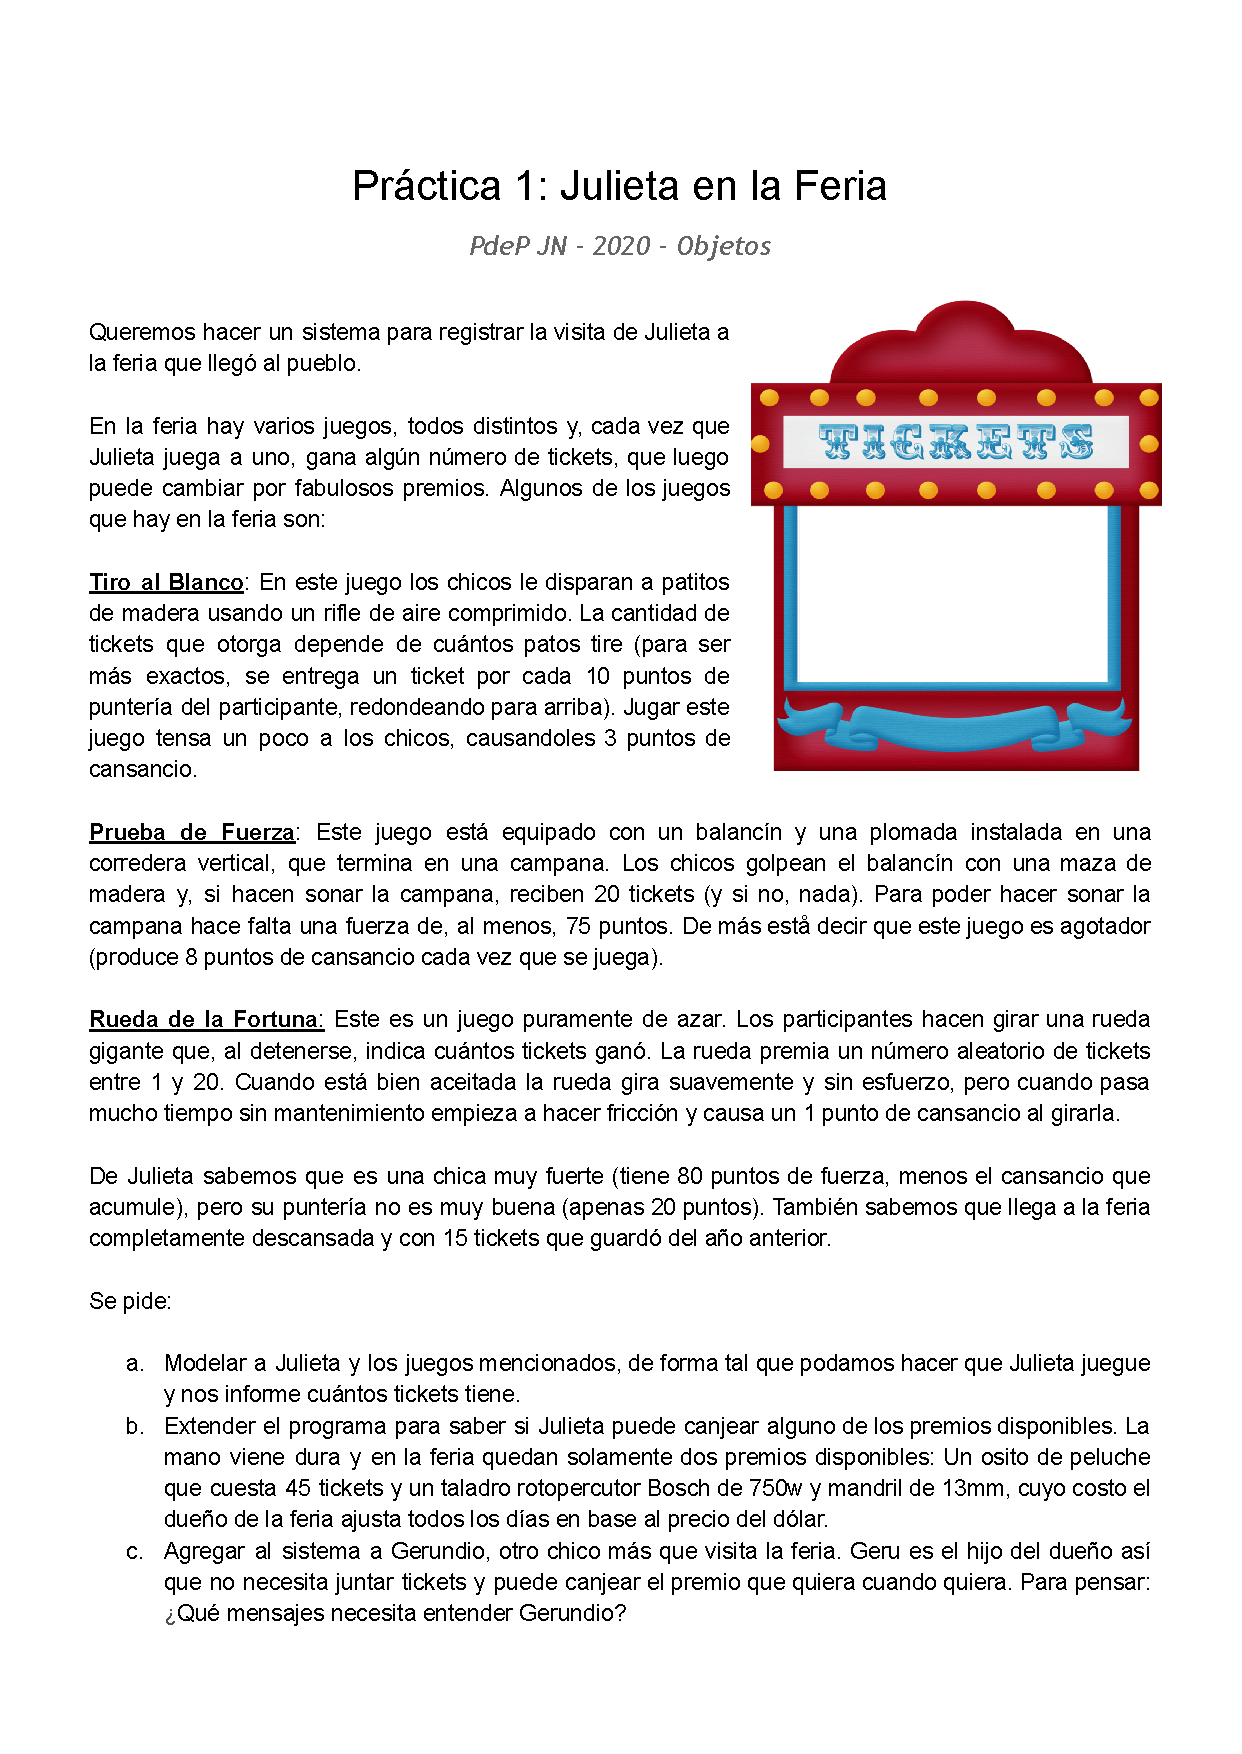
\includepdf[pages=-]{LaFeriaVideo18.pdf}
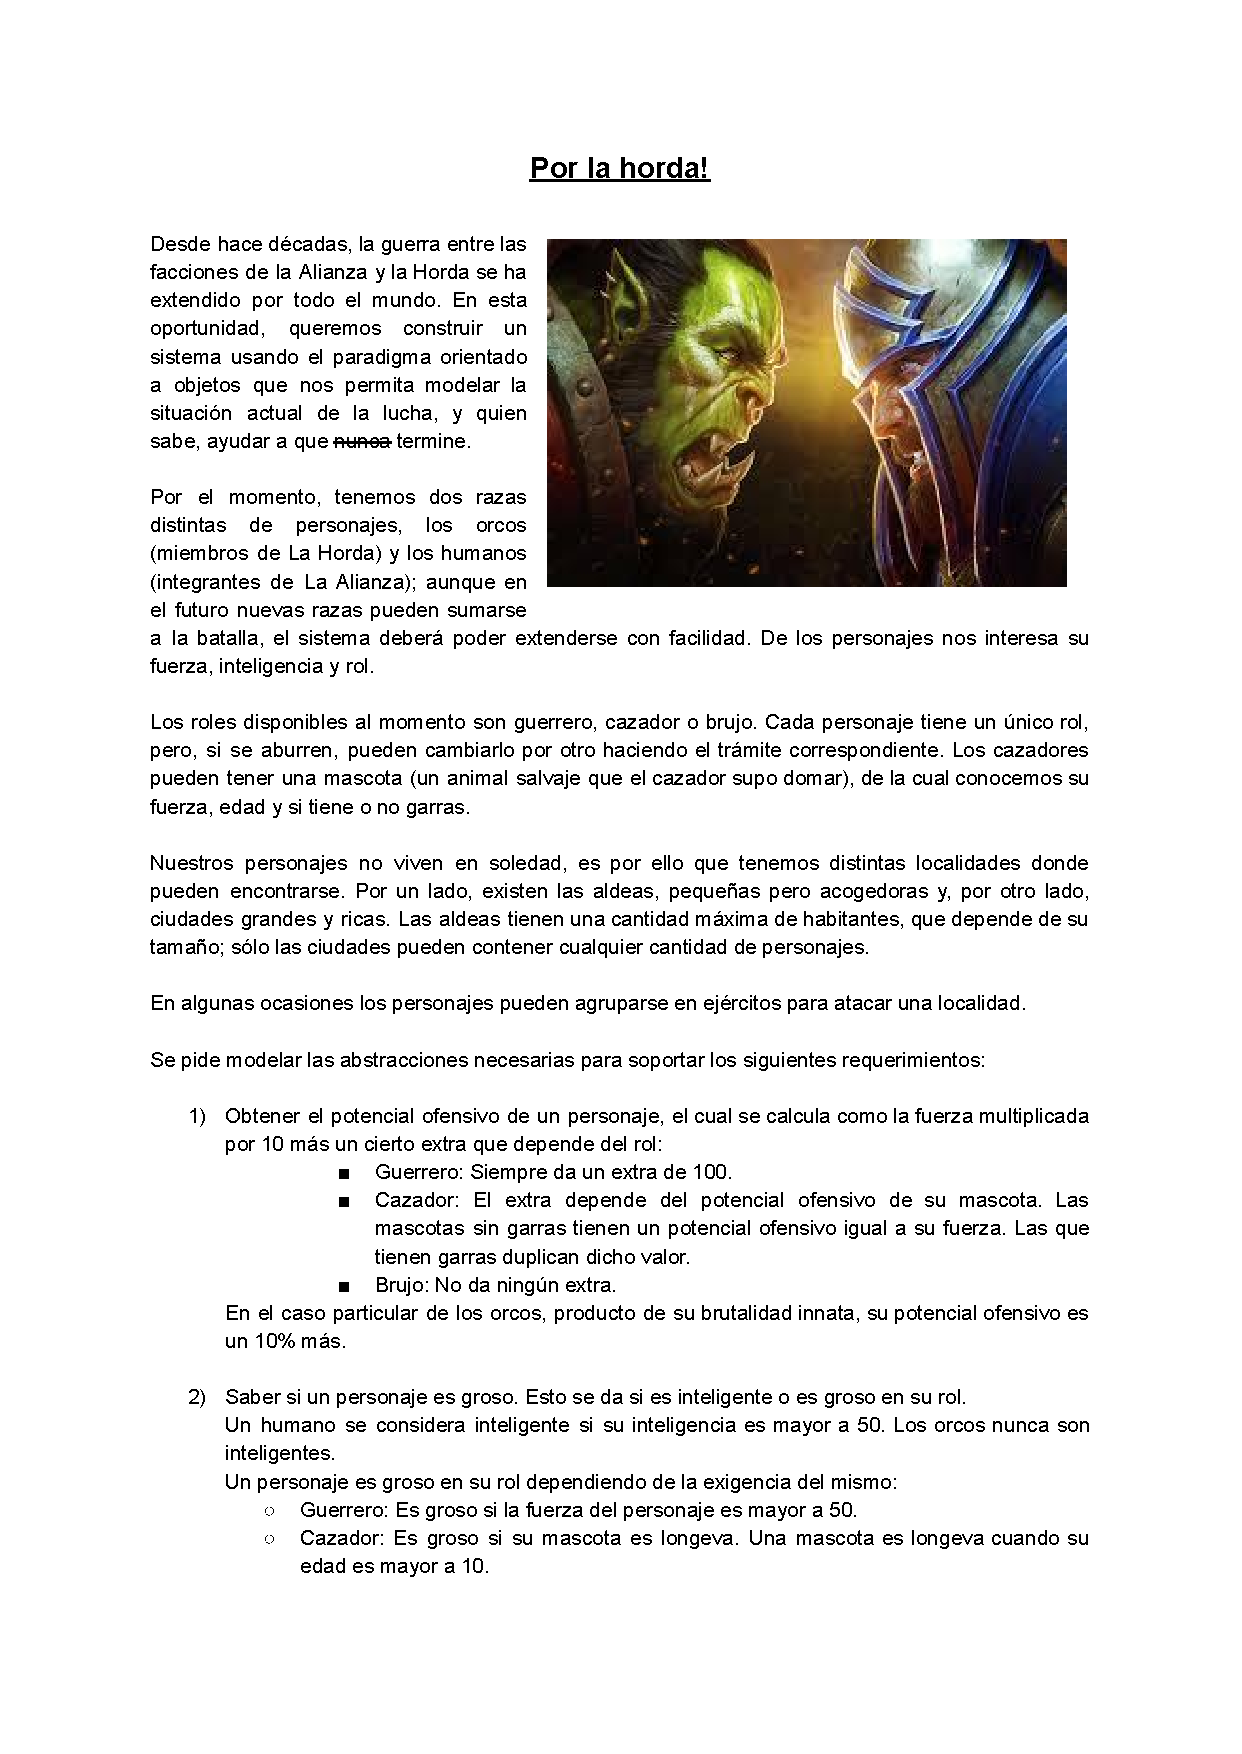
\includepdf[pages=-]{PorLaHordaVideo22.pdf}
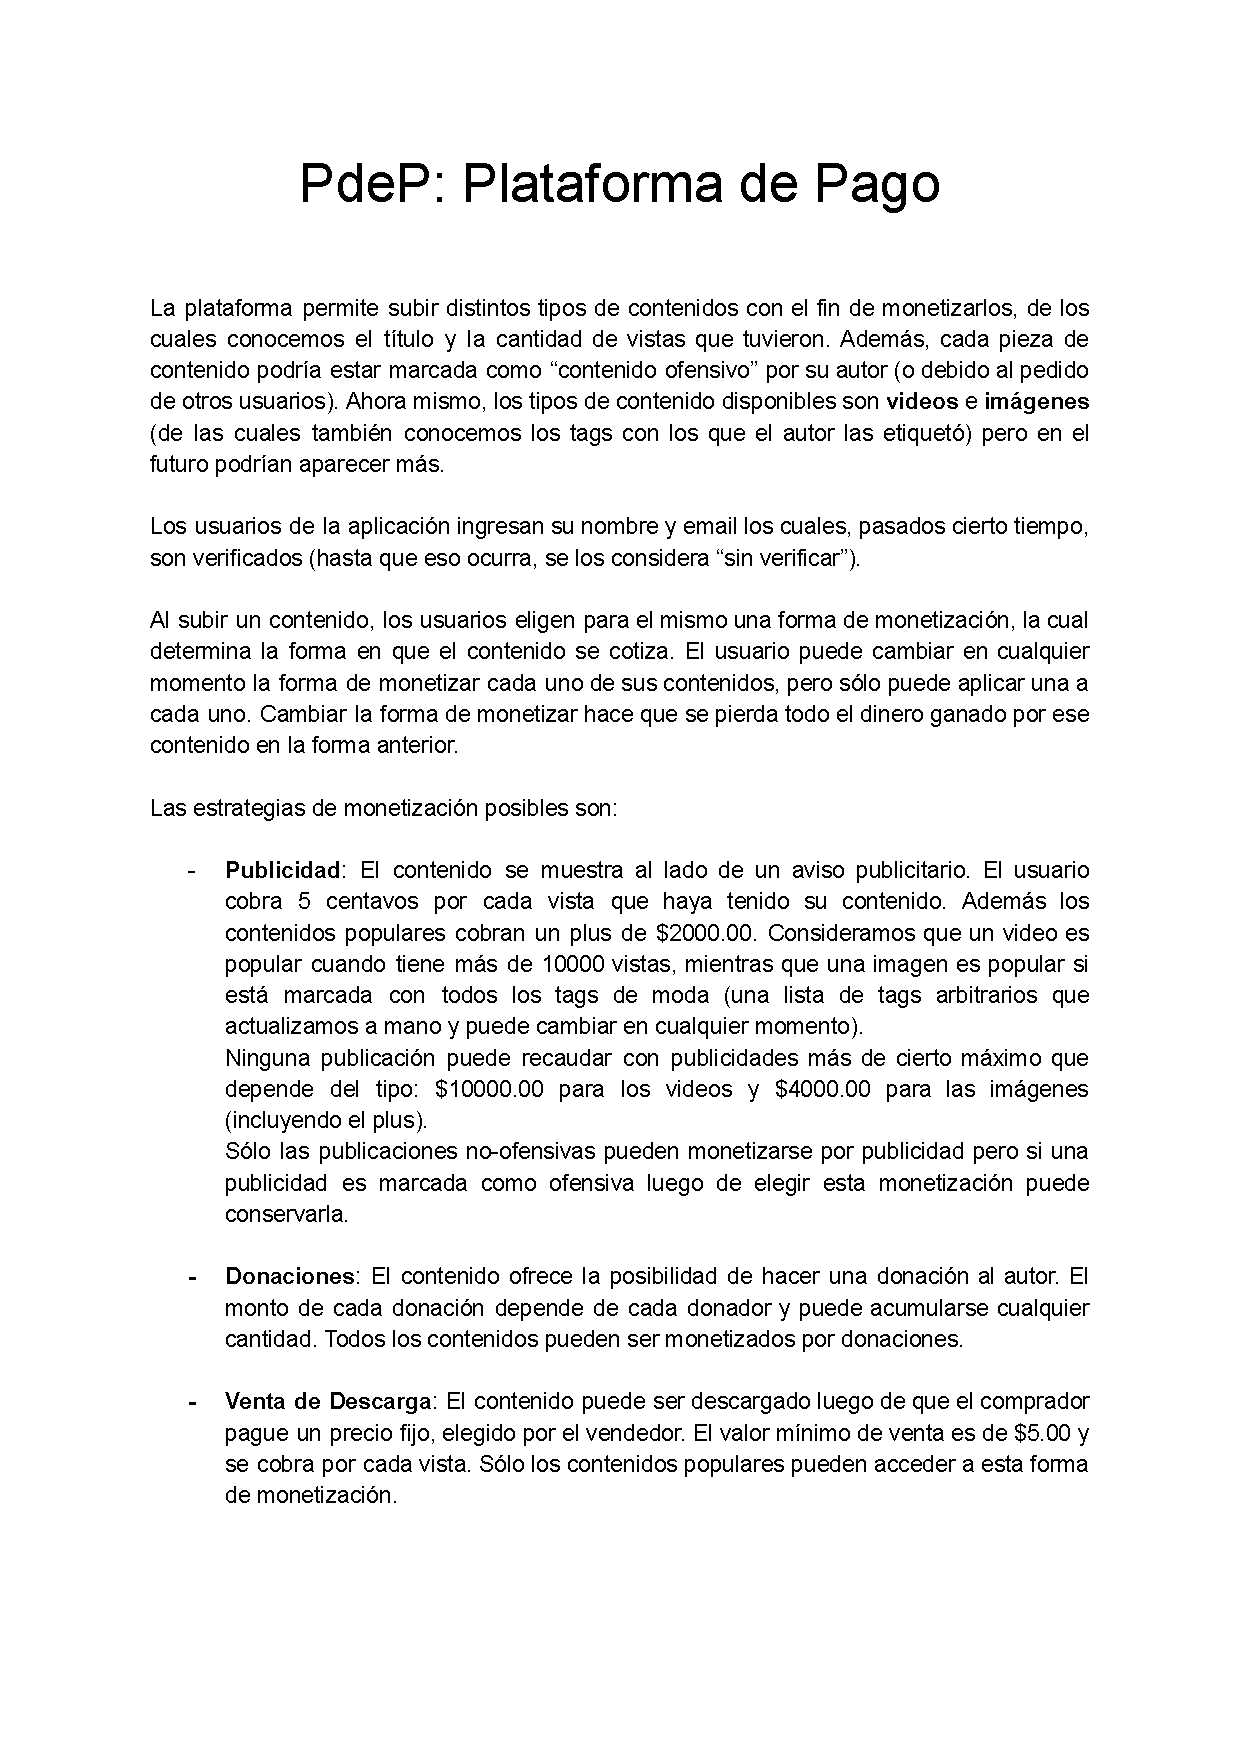
\includepdf[pages=-]{PdeP_ParcialObjetos_Monetizacion.pdf}
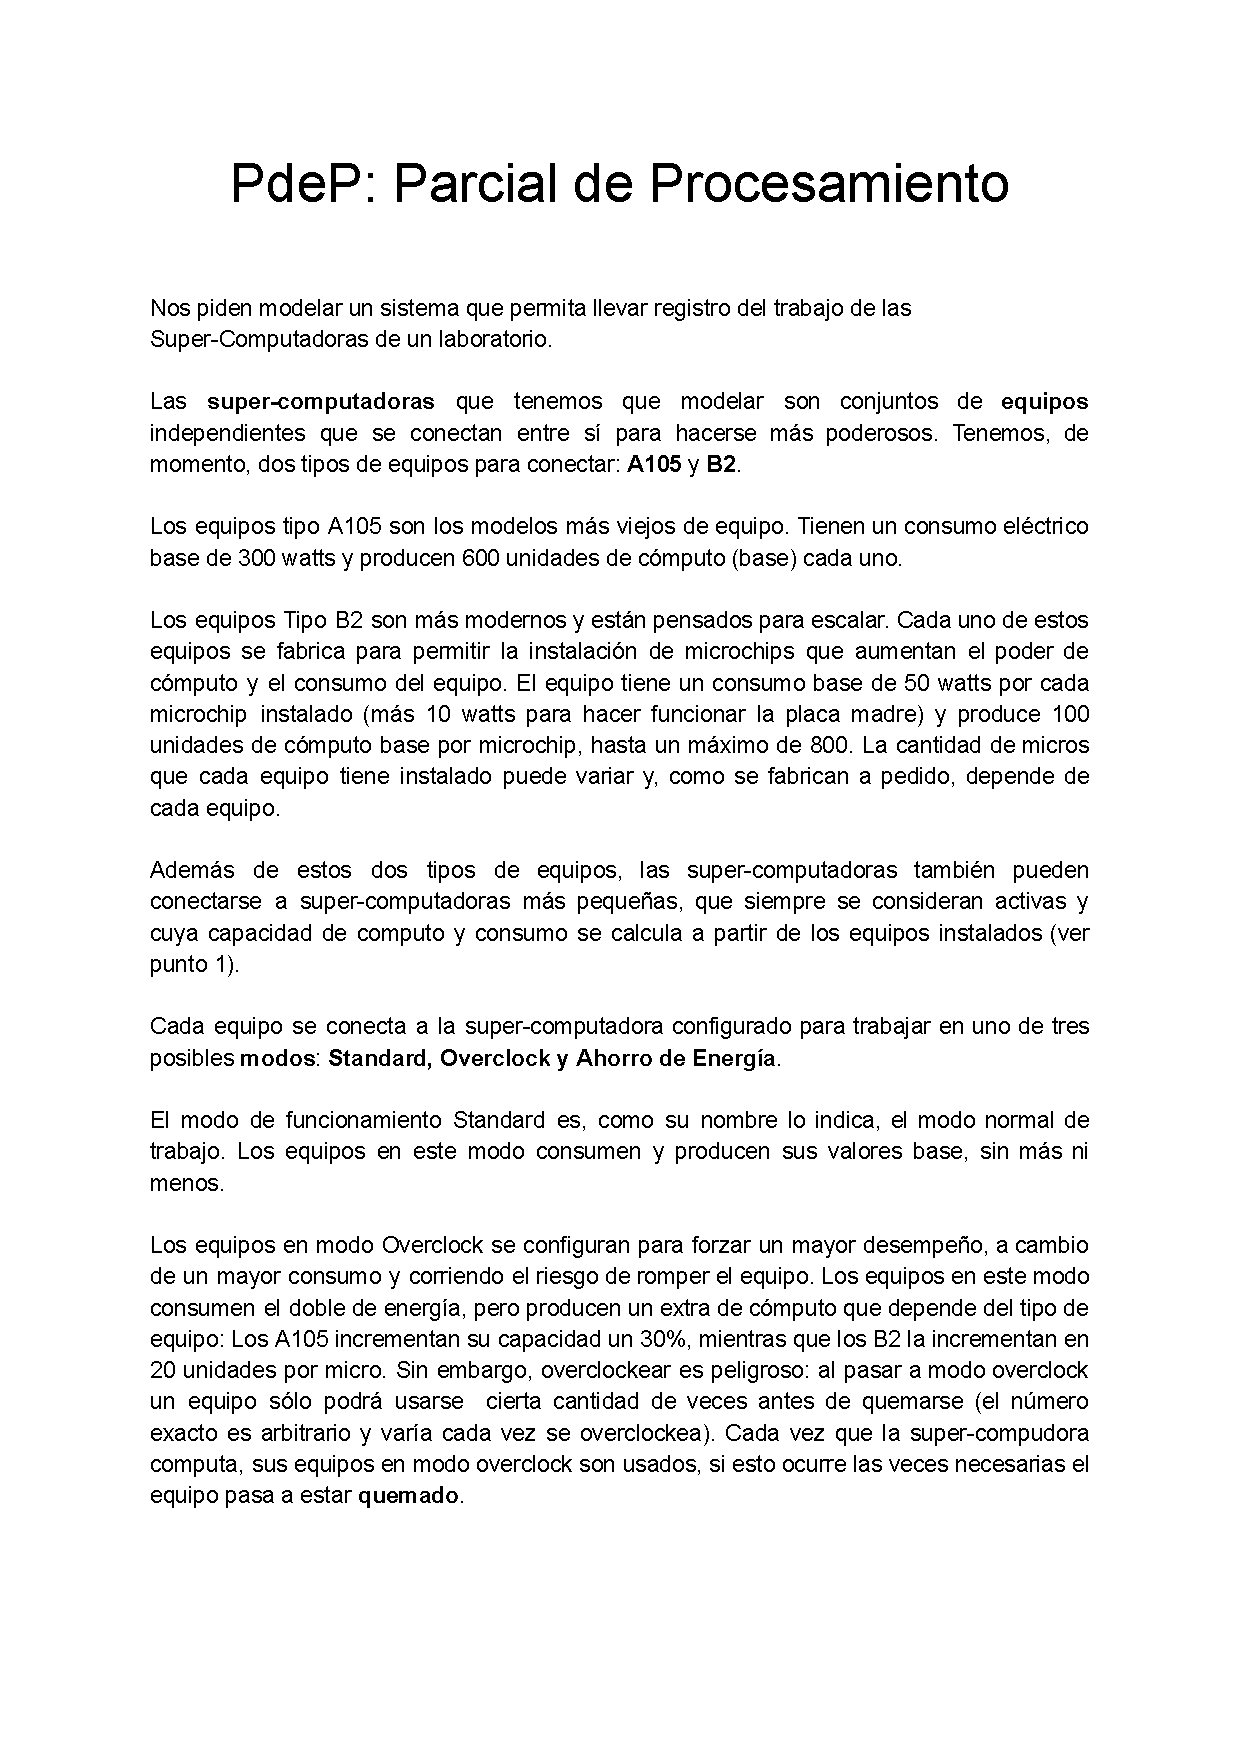
\includepdf[pages=-]{PdeP_Parcial_de_Pseudocomputadoras.pdf}
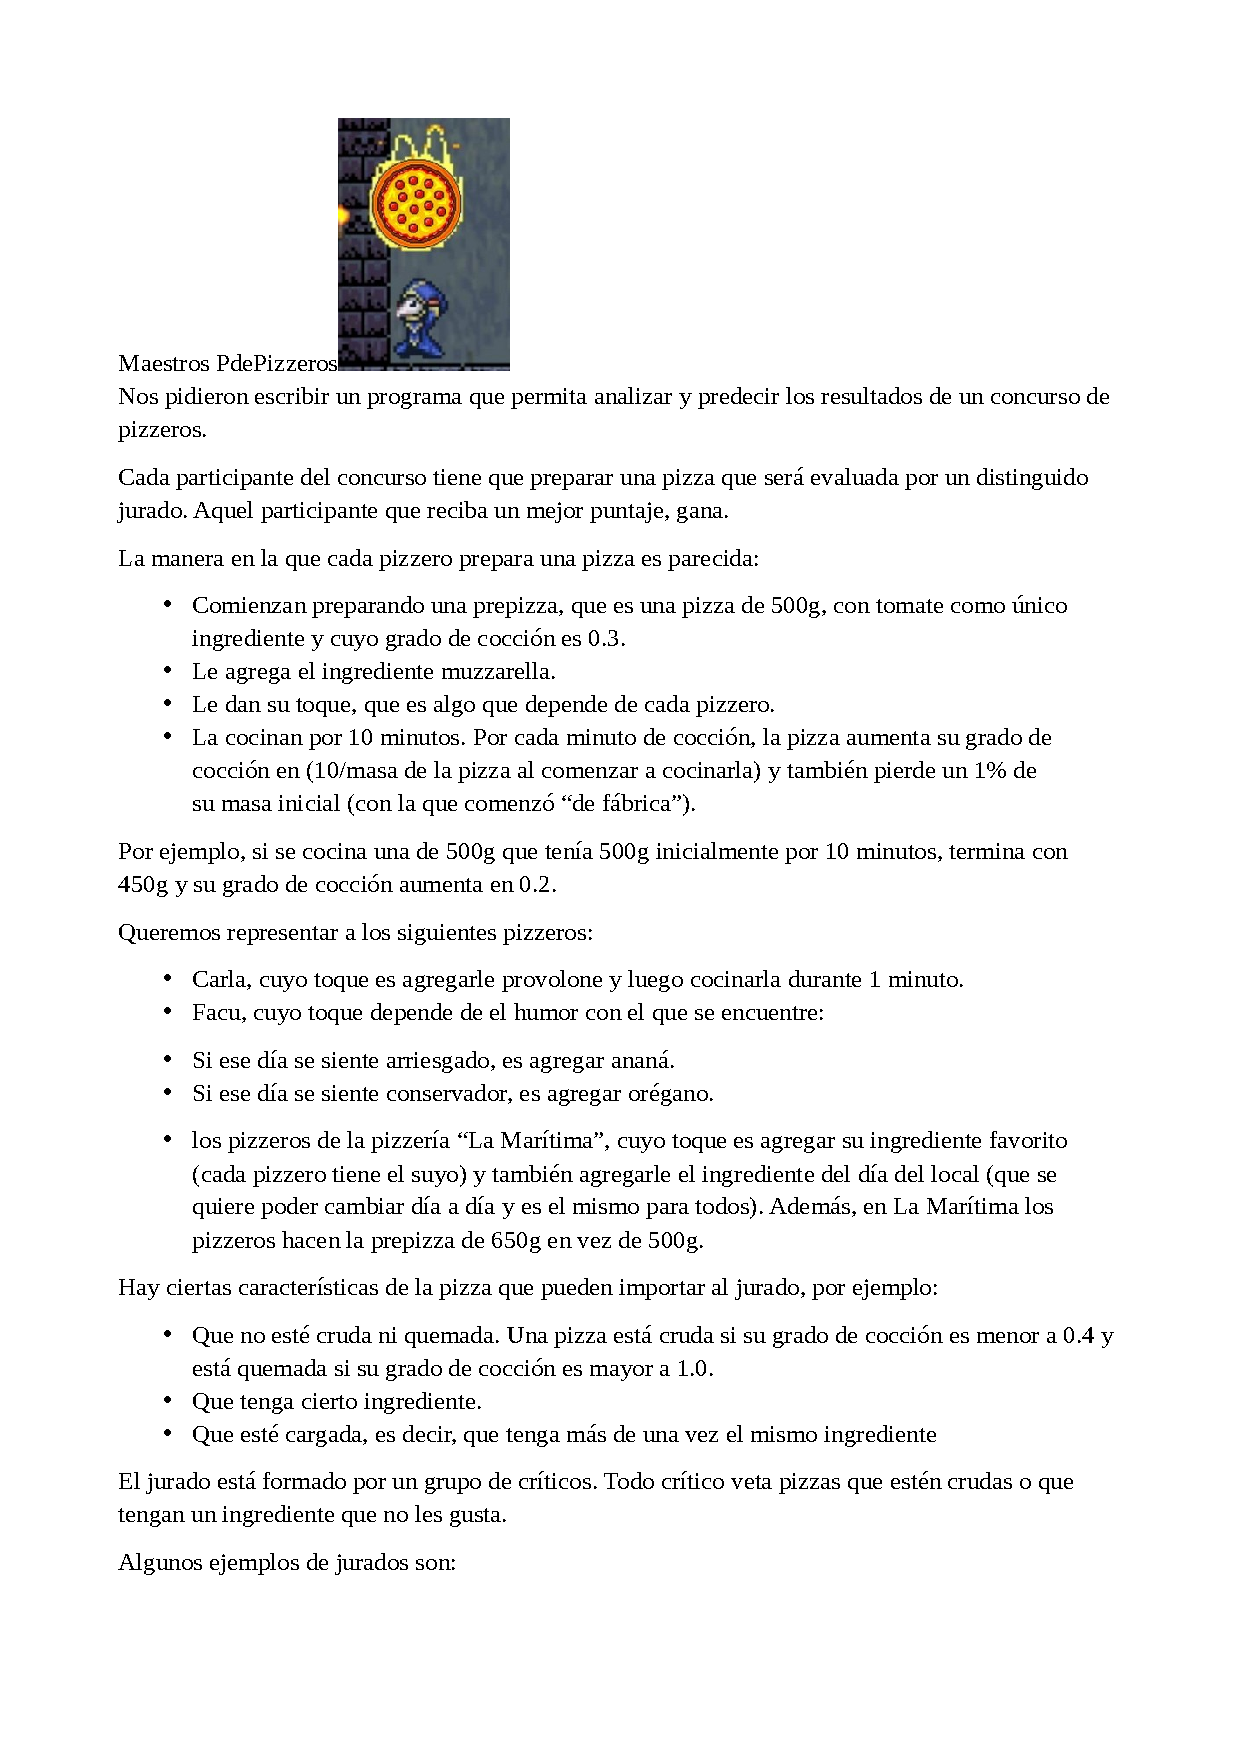
\includepdf[pages=-]{primerParcialPdePObjetos2023.pdf}



%\lstinputlisting[]{codigos/video17_e1_pepita/src/pepita.wlk}
%\lstinputlisting{codigo.asm}

\end{document}
